\section{Appendix}
\label{sec:appendix}

\subsection{Reproducibility}
\label{sec:appendix-repro}

Two infrastructure incidents occurred during this project and are recorded here rather
than omitted. During a repository root cleanup, an \texttt{ls -A} glob unintentionally
moved \texttt{.git}, \texttt{.omc}, and \texttt{\_\_pycache\_\_} alongside the
directories it was meant to reorganise; all three were restored and \texttt{git fsck}
reported no corruption. Separately, during a migration of run data to a second hard
drive, \texttt{rsync --remove-source-files} deleted the \texttt{tfevents} inodes of six
runs that were still training and writing to them; the open file handles were recovered
by copying from \texttt{/proc/<pid>/fd/N} for the twelve affected file descriptors, with
at most two minutes of logging lost per run. The first check performed after this
incident used a faulty grep pattern and incorrectly reported the runs as unaffected; we
record that false negative alongside the incident itself, since a reproducibility
appendix that omits it is worth less than none.

\subsection{Per-neuron firing intensity}
\label{sec:appendix-intensity}

\begin{figure}[t]
\centering
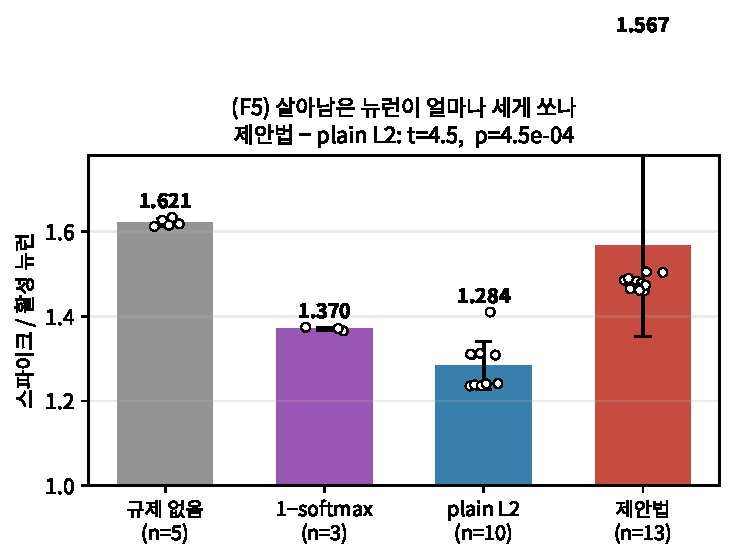
\includegraphics[width=\linewidth]{figures/f5_intensity_appendix.pdf}
\caption{Spikes per active neuron, ResNet-19/CIFAR-10, at the same
closest-landing pair used in Figure~\ref{fig:f2f3}. Bars are the
per-condition mean with individual runs overlaid; $n$ per condition is
given on the axis. Ours vs.\ Plain $L_2$: $t=10.5$, $p=8.4\times10^{-7}$.
As elsewhere in this section, the underlying active-neuron counts come
from \texttt{dead\_neuron\_ratio} measured over a 100-image batch -- not
a measurement of permanently silent neurons.}
\label{fig:f5_intensity}
\end{figure}

